%!TEX root = ../../thesis.tex

\chapter{Reassortment in Influenza Evolution}
\label{ch:influenza}

\section{Introduction}
\label{flu:introduction}

In this chapter, we study influenza virus, a common human pathogen with a substantial burden on human health.
Seasonal influenza epidemics have an annual mortality of between 250,000 and 500,000 \cite{WHO:2014b}.
Influenza pandemics, which have historically occurred roughly once every thirty years, can infect between 20-40\% of the global population.
For example, the Spanish influenza pandemic of 1918-1919 is estimated to have infected approximately 500 million people and lead to the death of between 50-100 million people \cite{Taubenberger:2006kl}.
This amounts to an infection of approximately 33\% of the population and a case fatality ratio of 5-6\% of global population.

The natural host reservoir of influenza is waterfowl.
Within this reservoir, several distinct subtypes circulate.
Subtypes are labeled by the antigenic type of two surface proteins, hemagglutinin (HA) and neuraminidase (NA).\footnote{An antigen is any molecule that elicits a host immune response. The adaptive immune system learns to recognize and protect against particular antigens. In order to evade the host immune response, the virus will mutate, giving rise to antigenic variation.}
There are presently eighteen types of HA (H1 to H18) and eleven types of NA (N1 to N11).
Zoonotic adaptations have led to multiple introductions to human populations, which have resulted in both isolated outbreaks and sustained transmission \cite{Nelson:2007bc}.\footnote{Understanding the genetic basis for host adaptation is an important and controversial research area. Our work in this area in collaboration with Yoshihiro Kawaoka is forthcoming \cite{Walters:2016a}.}

The evolution of influenza is punctuated by frequent reassortment.
Reassortment occurs when two virus particles coinfect the same host cell, and is a consequence of influenza having a segmented genome.
The result is viral progeny that carries genomic information from two independent parental strains.
This mode of evolution is known as \emph{antigenic shift}, because it can rapidly lead to antigenically distinct viral strains.\footnote{As opposed to \emph{antigenic drift}, due to random mutation and genetic drift.}
Antigenic shifts have historically led to major pandemics, which can occur when novel surface proteins reassort with internal segments already adapted to the human host.
Reassortments of this type led to Asian H2N2 flu pandemic of 1957 and the Hong Kong H3N2 flu pandemic of 1968 \cite{Lindstrom:2004il}.
The 2009 H1N1 pandemic strain emerged from a triple reassortment between avian, swine, and human circulating strains \cite{Hernandez:2011ud,Smith:2009io}.
The pandemic had a global infection rate of between 11\%-21\% but a lower mortality rate than initially expected.\footnote{The 2009 H1N1 pandemic is an excellent example of the delicate balance between virulence and transmissibility.}
The 2013 H7N9 flu outbreak was caused by a triple reassortment of three distinct avian strains \cite{Chen:2013kp}.
Traditionally, reassortments have been identified by hand, by comparing phylogenetic trees constructed from different genomic segments \cite{Nelson:2006bx}.

Recent years have seen increased concerns about the pandemic potential for zoonotic adaptation of highly pathogenic strains of influenza.
Of particular concern is H5N1, which has an estimated case fatality rate of 50\% (449 deaths from 846 confirmed human cases) \cite{WHO:2016a}, but has so far not exhibited sustained person-to-person transmission \cite{WHO:2014b}.
Studies in ferret models demonstrated sustained transmission in a reassortent H5N1 with as few as four mutations in the HA protein \cite{Imai:2012hn}.
These concerns underscore the need to efficiently characterize and represent reticulate evolution in influenza.
Since the 2009 H1N1 pandemic, substantial effort has been put into collecting and organizing fully sequenced influenza genomes.
The NCBI Influenza Virus Resource now contains over 400,000 unique viral isolates \cite{Bao:2008cq}.
The large quantity of genomic data that has been collected provides an ideal environment for studying reticulate evolution with high resolution.

\section{Influenza Virology}
\label{flu:virology}

Influenza is an enveloped single-stranded negative-sense RNA virus of family Orthomyxoviridae.
The virus has a segmented genome with eight segments coding for eleven proteins.
The genome length is approximately 13.5~kb.
The viral structure is shown in Figure~\ref{fig:flu:genome}.
The segments are typically ordered from longest to shortest and are detailed in Table~\ref{table:influenza_genome_segments}.
Of these segments, hemagglutinin (HA) and neuraminidase (NA) are the two most important.
HA and NA form the two surface protein markers and are responsible for viral entry and release.
HA regulates host cell binding and entry into host epithelial cells.
HA is the strongest determinant of host specificity: different hosts express different sialic acid types.
Avian influenza binds to type 2-3 sialic acid receptors, while human influenza binds to type 2-6 sialic acid receptors.
NA is the surface protein that cleaves the newly replicated virus particles from the cell surface.
Together, HA and NA determine the strain subtype and are a primary marker of host specificity and transmissibility.
PA, PB1, and PB2 form a polymerase complex and are involved in viral replication.
Mutations in these proteins can be among the most important in determining host adaptation and virulence, particularly mutation PB2--E627K, \cite{Subbarao:1993tt,Hatta:2001cw}. 
The remaining proteins, including NP, M1, M2, and NS1 are largely structural proteins involved in capsid formation and viral packaging.

\begin{table}
\centering
\caption{Influenza Protein Segments}
\small
\setlength{\aboverulesep}{0pt}
\setlength{\belowrulesep}{0pt}
\setlength{\extrarowheight}{.75ex}
\begin{tabularx}{\textwidth}{XXXX}
\toprule\rowcolor{gray!50}
Segment Number & Segment Name & Protein & Length (aa) \\
\midrule
                   1 & Polymerase basic 2 & PB2 & 759 \\
\rowcolor{gray!25} 2 & Polymerase basic 1 & PB1 & 757 \\
                   3 & Polymerase acidic  & PA  & 716 \\
\rowcolor{gray!25} 4 & Hemagglutinin      & HA  & 563 \\
                   5 & Nucleoprotein      & NP  & 498\\
\rowcolor{gray!25} 6 & Neuraminidase      & NA  & 470\\
\multirow{2}{*}{7} & \multirow{2}{*}{Matrix}  & M1  & 252 \\
				   &                          & M2  & 97 \\
\rowcolor{gray!25}                      &                                 & NS1 & 230 \\
\rowcolor{gray!25} \multirow{-2}{*}{8}  & \multirow{-2}{*}{Nonstructural} & NS2 & 121 \\
\bottomrule
\end{tabularx}
\label{table:influenza_genome_segments}
\end{table}

\begin{figure}
\begin{center}
\centerline{\includegraphics[width=.5\columnwidth]{./fig/influenza/flu_genome.jpg}}
\caption[Structure of an influenza virus particle]{Structure of an influenza virus particle. Surface antigens HA and NA coat this surface and are involved in viral entry and exit into the host cell. The surface capsid is formed from matrix proteins M1 and M2. PB1, PB2, and PA form a polymerase complex assisting in viral replication in the infected cell.}
\label{fig:flu:genome}
\end{center}
\end{figure}

\section{Influenza Reassortment}
\label{flu:reassortment}

We characterized reassortment in avian influenza using persistent homology.
We first compiled an aligned dataset of 3,105 complete avian influenza genomes from the NIH Influenza Sequence Database.
These sequences span in time from 1956 to 2012. 
We collected samples from all influenza subtypes.
The majority of our sequences are of the H5 and H6 type, with a smaller proportion of H3, H7, and H9.
The distribution of collected HA types and years is shown in Figure~\ref{fig:flu:histograms}.

\begin{figure}
\centering
\includegraphics[]{fig/influenza/flu_histograms.pdf}
\caption[Influenza Dataset Statistics]{The avian influenza dataset analyzed in this chapter. Sequences spanned from 1950 to 2011, with the vast majority being collected after 2000. Most sequences were of HA type H5, with H6 and H3 following. Dataset was collected from the NCBI Influenza Virus Resource \cite{Bao:2008cq}}
\label{fig:flu:histograms}
\end{figure}

We first applied persistent homology to each genomic segment individually, as shown in Figure~\ref{fig:flu:segment_barcodes}.
Here we see very little higher homology, consistent with no intra-segmental recombination.
The presence of higher homology is likely due to back mutation, which is expected to be more common in viruses with high mutation rates and shorter genomes (i.e. the infinite sites model does not hold).
However, an analysis of the concatenated full genome reveals a complex topology, with a large number of homological invariants in one and two dimensions (Figure~\ref{fig:flu:concatenated_genome_barcode}).

These results show that persistent homology can detect pervasive reassortment in influenza.
One-dimensional $\ICR$ provides a lower-bound estimate of reassortment rate.
We calculate $\ICR < 1$ event per year for classic H1N1 swine and H3N2 human influenza, supported by previous phylogenetic estimates \cite{Lycett:2012fqa,Holmes:2005cia}.
In contrast, we calculate a much higher rate of 22.16 reassortments per year for avian influenza A.
This difference could be explained by the high diversity and frequent coinfection of avian viruses \cite{Lubeck:1979ws} and correlates with the high proportion of avian reassortants reported in previous studies \cite{Dugan:2008iba}.

\begin{figure}
\centering
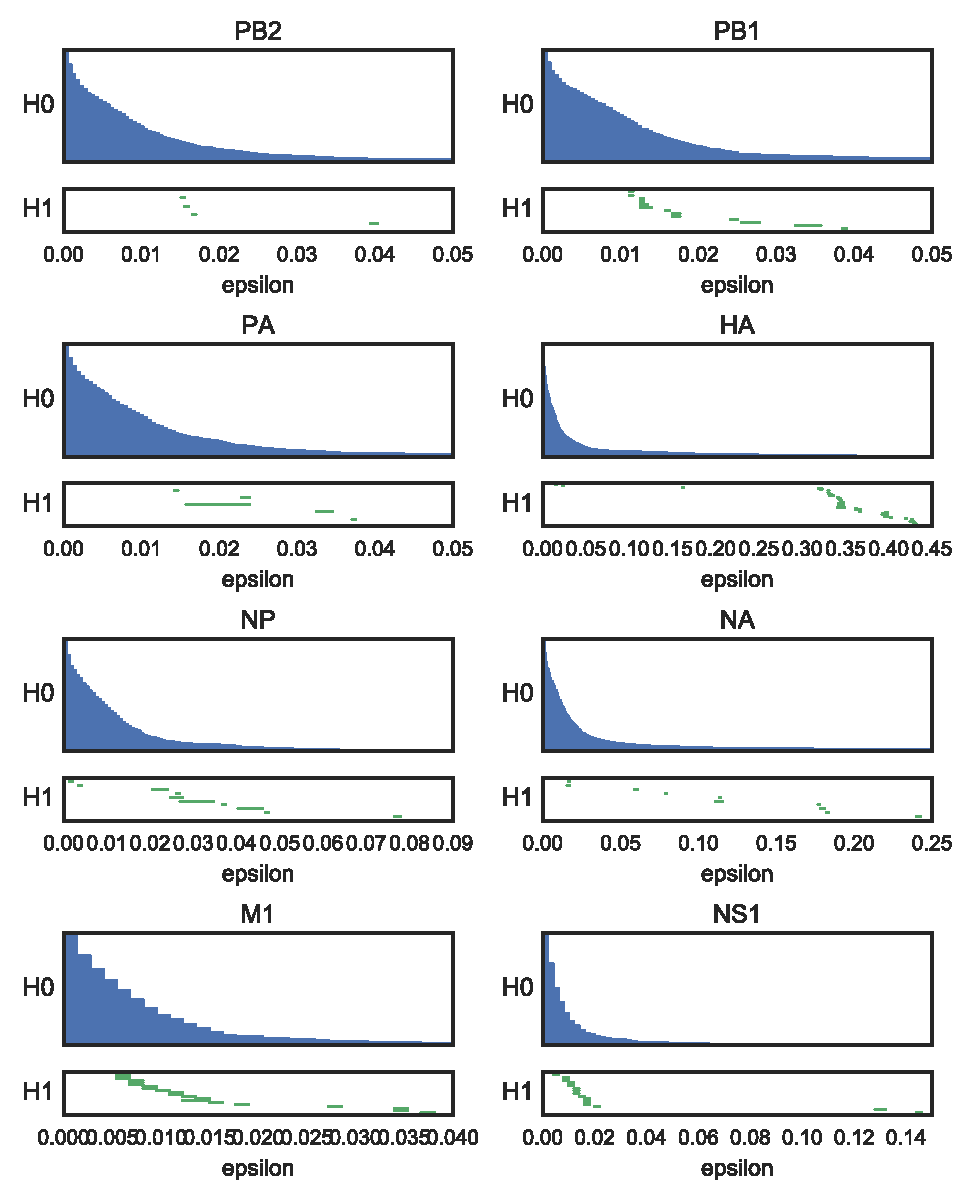
\includegraphics[]{fig/influenza/flu_segment_barcodes.pdf}
\caption[Influenza Genome Segment Barcodes]{Influenza Genome Segment Barcodes. Persistent homology computed on a per-segment basis reveals very little $H_1$ homology, indicating limited intrasegment reticulation.}
\label{fig:flu:segment_barcodes}
\end{figure}

\begin{figure}
\centering
\includegraphics[]{fig/influenza/flu_concat_barcode.pdf}
\caption[Influenza Concatenated Genome Barcode]{Influenza Concatenated Genome Barcode. Persistent homology computed on the full concatenated genome reveals substantial $H_1$ and $H_2$ homology, indicating high levels of reticulate exchange.}
\label{fig:flu:concatenated_genome_barcode}
\end{figure}

We used mapper to visualize the relationships in our influenza dataset.
A series of mapper networks is shown in Figure~\ref{fig:flu:networks_by_subtype}.
The networks were generated using a Hamming metric and the first and second MDS components as a 2D lens.
In each subfigure we color the network by influenza subtype, for the top ten subtypes represented in the dataset.
We can see that the current classification of flu sequences by HA and NA type is a reasonable approach, as flu isolates of the same subtype tend to cluster together tightly within the network.
H6N2 is the sole subtype to be represented by two clusters in the network.
When we examined the members of each H6N2 cluster, we found that both consisted of isolates spanning long time frames, suggesting that multiple stable lineages of H6N2, each carrying different internal segments, have persisted.

% The Mapper representation offers further resolution into isolate relationships that can account for whole genomes.
% We performed an MCL clustering of the network and considered how subtype-pure each cluster was.
% \kje{TODO: Make the figure and expand here. Explain alternate classification scheme.}

\begin{figure}
\centering
\includegraphics[width=\textwidth]{fig/influenza/flu_networks_by_subtype.pdf}
\caption[Influenza Networks By HA Subtype]{Influenza Networks By HA Subtype. The networks were generated using Ayasdi using a Hamming metric and a 2D MDS coordinate lens. Lens parameters were (gain=5, resolution=40, equalize=False).},
\label{fig:flu:networks_by_subtype}
\end{figure}

\section{Nonrandom Association of Genome Segments}
\label{flu:nonrandom_reassortment}

We observed nonrandom association of flu segments.
Statistical inference on the loops corresponding to reassortments identified segments that tend to co-segregate with each other during reassortment.In particular, polymerases co-segregate, while genes coding for envelope and capsid proteins show independent reassortment patterns.
Cosegregation of polymerases suggests that effective protein–protein interaction between the polymerase complex and the NP protein constrain reassortment. 

Although previous phylogenetic studies confirmed a high reassortment rate in avian influenza, none has identified a clear pattern of gene segment association \cite{Dugan:2008iba}.
To determine whether any segments cosegregate more than expected by chance, we considered all pairs of concatenated segments and estimated the number of reassortments using $b_{1}$.
We then ascertained the significance of observing a number of reassortments between each pair of segments given the total estimate of reassortments in the concatenated genome.
These patterns of cosegregation are represented in Figure~\ref{fig:flu:nonrandom_reassortment}, in which thicker edges indicate cosegregation, as measured by a lower level of homology between segment pairs.
% \kje{TODO: Put statistics in a table}
Analysis of avian influenza reveals a statistically significant configuration of four cosegregating segments: polymerase basic 2 (PB2), polymerase basic 1 (PB1), polymerase acidic (PA), and nucleoprotein (NP).
Interestingly, this pattern mimics previous in vitro results that suggest that effective protein-–protein interaction between the polymerase complex and the NP protein constrain reassortment \cite{Lubeck:1979ws}.

\begin{figure}
\begin{center}
\centerline{
\includegraphics[width=\columnwidth]{./fig/influenza/flu_reassortment_correlations.pdf}}
\caption[Influenza Nonrandom Reassortment]{Influenza Nonrandom Reassortment}
\label{fig:flu:nonrandom_reassortment}
\end{center}
\end{figure}

\section{Multiscale Flu Reassortment}
\label{flu:multiscale_reassortment}

We computed persistent homology on the avian influenza sequences across the seven major HA subtypes.
The persistence diagram is shown in Figure \ref{fig:flu:scatterplot}, along with density estimates for the birth and death distributions.
Both birth and death times appear strongly bimodal, unlike in the coalescent simulations, which were strictly unimodal.
This suggests two distinct scales of topological structure.
Using the representative cycles output by Dionysus on a subset of this data, we classified features as intrasubtype (involving one HA subtype) and intersubtype (involving multiple HA subtypes).
The $H_1$ barcode diagram for this data is shown in the Figure \ref{fig:flu:scatterplot} inset.
Intrasubtype features, in blue, occur at an earlier filtration scale than intersubtype features, in green.
The multiscale topological approach of persistent homology can distinguish biological events occuring at different genetic scales.

We isolated the two peaks and estimated two recombination rates: an intrasubtype $\rho_{1}=9.68$, and an intersubtype $\rho_{2}=21.43$.
We conclude that intersubtype recombination occurs at a rate over twice that of intrasubtype recombination, however a genetic barrier exists that maintains distinct subtype populations.
The nature of this barrier warrants further study.
This illustrates a real-world example in which multiscale topological structure can be captured by persistent homology and given biological interpretation.

\begin{figure}
\centering
\includegraphics[width=\columnwidth]{./fig/influenza/flu_scatterplot.pdf}
\caption[$H_1$ persistence diagram computed from an avian influenza dataset.]{The $H_1$ persistence diagram computed from an avian influenza dataset. On the top and left are plotted the marginal distributions of birth and death times, along with a density estimate for each distribution. The bimodality indicates two scales of topological structure. Inset: The barcode diagram for a subset of this data. Blue bars have representative cycles involving only one subtype, green bars have cycles involving multiple subtypes.}
\label{fig:flu:scatterplot}
\end{figure}

\section{Conclusions}
\label{flu:conclusions}

In this chapter we analyzed reassortment patterns in influenza.
The segmented nature of the influenza genome, and the large amount of collected genome information, make influenza ideal for the application of topological methods.
Reassortment occurs when a single cell is coinfected by multiple strains of the virus, and can lead to the emergence of novel pandemics.
Current methods of classifying influenza, based solely on HA and NA subtype, fail to account for information in the internal segments and there is at present no consistent methodology for dealing with reassortments.
We have applied methods from TDA to characterize both the scale and frequency of reassortment in influenza, estimating both reassortment rates and cosegregation patterns.
Using Mapper, we determined classifications of viruses based on whole genome information that provide a higher resolution picture into extant circulating strains.
Further, from the persistence diagram we identified a bimodal structure of $H_1$ invariants, which suggests a genetic barrier maintaining subtype diversity.